% -*- root: warwickthesis.tex -*-

\section{Mathematical background}
\label{sec:math-backgr}

This section contains the important basic principles we use to investigate biological systems. We start off by examining Markov chains and introduce basic principles for discrete time and continuous time Markov chains. They  are an essential part of the model introduced in Chapter \ref{cha:stamm} and applied in later chapters. Then in Section \ref{sec:hmm} we introduce the slightly more involved hidden Markov models, which are often applied to biological systems and have similarities to the aggregate Markov chains introduced in Chapter \ref{cha:stamm}. Section \ref{sec:least-squares} contains a brief presentation of the estimation procedure used in our investigation. This is followed in Section \ref{sec:penalisation} by a discussion on regularisation during estimation in which two procedures penalizing for large parameter values and overfitting commonly used to regularise estimated parameters are outlined. The concept of identifiability, which can be of importance in estimation is defined in Section \ref{sec:identifiability-back}. Then we move on to a discussion on model selection in Section \ref{sec:model-selection-1} and various techniques for distinguishing between models. Finally, in Section \ref{sec:monte-carlo-integr} a very useful numerical tool is presented for integrating functions where a closed form solution is not possible. This method is employed in the second model put forward in Chapter \ref{cha:cell-cycle} of this thesis.

\subsection{Markov chains}
\label{sec:markov-chains}

In physics prior to the advent of statistical physics and quantum mechanics in the early 20th century, the world was modelled as deterministic. Of course, we now know that despite many aspects of the observable world being deterministic there is an even larger set of objects which does not lend itself to a deterministic description. Objects or ideas that can be described using deterministic principles do at times derive from non-deterministic effects cancelling out or being only important at a different scale. Stochastic processes are used to describe systems where deterministic principles fail. A concept shared by many such systems is that they are evolving with a time dependent stochastic part. One of the first attempts to describe such a system was the modelling of Brownian motion by \cite{Einstein:2005ww}, which paved the way for further research on this topic. Here we start by defining some variables and simple principles governing one simple model that has found widespread application, the Markov chain model.

\subsubsection{Discrete time}

Let $X(t)$ be a time dependent continuous random variable and $x(t_1), x(t_2) \ldots $ are observations at discrete $t_1, t_2, \ldots$. We write probability densities as $p$ and the joint probability density is written as $p(X(t_1) = x(t_1), X(t_2) = x(t_2) \ldots)$. In addition we can also write the probability density of a set of observations at $t_1, t_2, \ldots$ conditional on observations at $\tau_1, \tau_2, \ldots $ as:

\begin{equation}
  \label{eq:stoch-joint-init}
  p(X(t_1) = x_1, X(t_2) = x_2\ldots | X(\tau_1 ) = x^{\prime}_1, X(\tau_2) = x^{\prime}_2 \ldots).
\end{equation}
where $x^{\prime}_1 \neq x_1$ and is used to distinguish the two. The model we wish to consider is a special case of a stochastic process: a \emph{Markov chain}. The most important principle underlying a Markov chain is the \emph{Markov assumption} and it can be written in terms of the conditional probability density. We introduce the notation of the current state at $t_n$ of a system as $x_n$ with a continuous state space and discrete time; if we now write the probability density of this measurement conditional on all preceding measurements $x_{n-1}, x_{n-2}, \ldots x_1$ the following principle must hold:

\begin{multline}
  \label{eq:stoch-joint}
  p(X(t_n)=x_n | X(t_{n-1}) = x_{n-1}, X(t_{n-2}) =x_{n-2}, \ldots X(t_1)=x_1 \ldots) = \\ p(X(t_n)=x_{n}| X_{n-1} = x_{n-1}),
\end{multline}
this is also known as the Markov property and it states, an observation is only conditionally dependent on the observation immediately preceding it. Further, the Markov property eqn. (\ref{eq:stoch-joint}) and an initial distribution $ p(1) = p(X(t_1) = x_1)$ uniquely determines a Markov chain in discrete time and with a discrete state space. This only holds because any joint probability can be written as a product of subsequent transition probabilities starting from the initial distribution. If we now write the transition probability as $p_{ij}$ as the transition from state $i$ to state $j$ (or as $P$ in matrix notation) we can write the distribution of a Markov chain at time $t$, $p(t)$ where $t \in \mathbb{N}$ as:

\begin{equation}
  \label{eq:markov-chain}
  p(t) = p(1)P^t.
\end{equation}

\subsubsection{Continuous time}
\label{sec:continous-time}

If we extend the Markov chain to continuous time but keep the state space discrete, we have to introduce the generator matrix $G$. It uniquely defines a continuous time Markov chain together with the initial distribution similar to a  discrete time Markov chain. The entries in the generator matrix are the transition rates from state $i$ to state $j$ satisfying $g_{i,j} \geq 0$. Diagonal entries of the matrix are $g_{i,i} = - \sum_{j \neq i} g_{i,j}$. We can now write the time evolution as

\begin{equation}
  \label{eq:mc-time-ev}
  \frac{d}{dt} P(t) = G\, P(t) = P(t)\, G,
\end{equation}
which are known as the backward and forward equation respectively, where $P(t)$ is a matrix with the entries $p_{ij}(t)$. If we are now interested in the state occupation as a function of time $p(t)$ and define $p(t=0)$ as the initial state distribution we can use eqn. (\ref{eq:mc-time-ev}) and write

\begin{equation}
  \label{eq:state-occ-back}
  \frac{d}{dt}p(t) = p(0) \frac{d}{dt} P(t) = p(0) P(t) G = p(t)G.
\end{equation}
It is often useful to rewrite eqn. (\ref{eq:state-occ-back}) element wise form using the definition of the generator matrix such that

\begin{equation}
  \label{eq:mc-master}
  \frac{d}{dt} p (t) = \sum_{j\neq i} \left( p_j(t)g_{j,i} - p_i(t)g_{i,j} \right),
\end{equation}
which is known as the Master equation and is useful in allowing us to derive many results for Markov chains.

\subsection{HMM}
\label{sec:hmm}

\begin{figure}[!t]
\centering
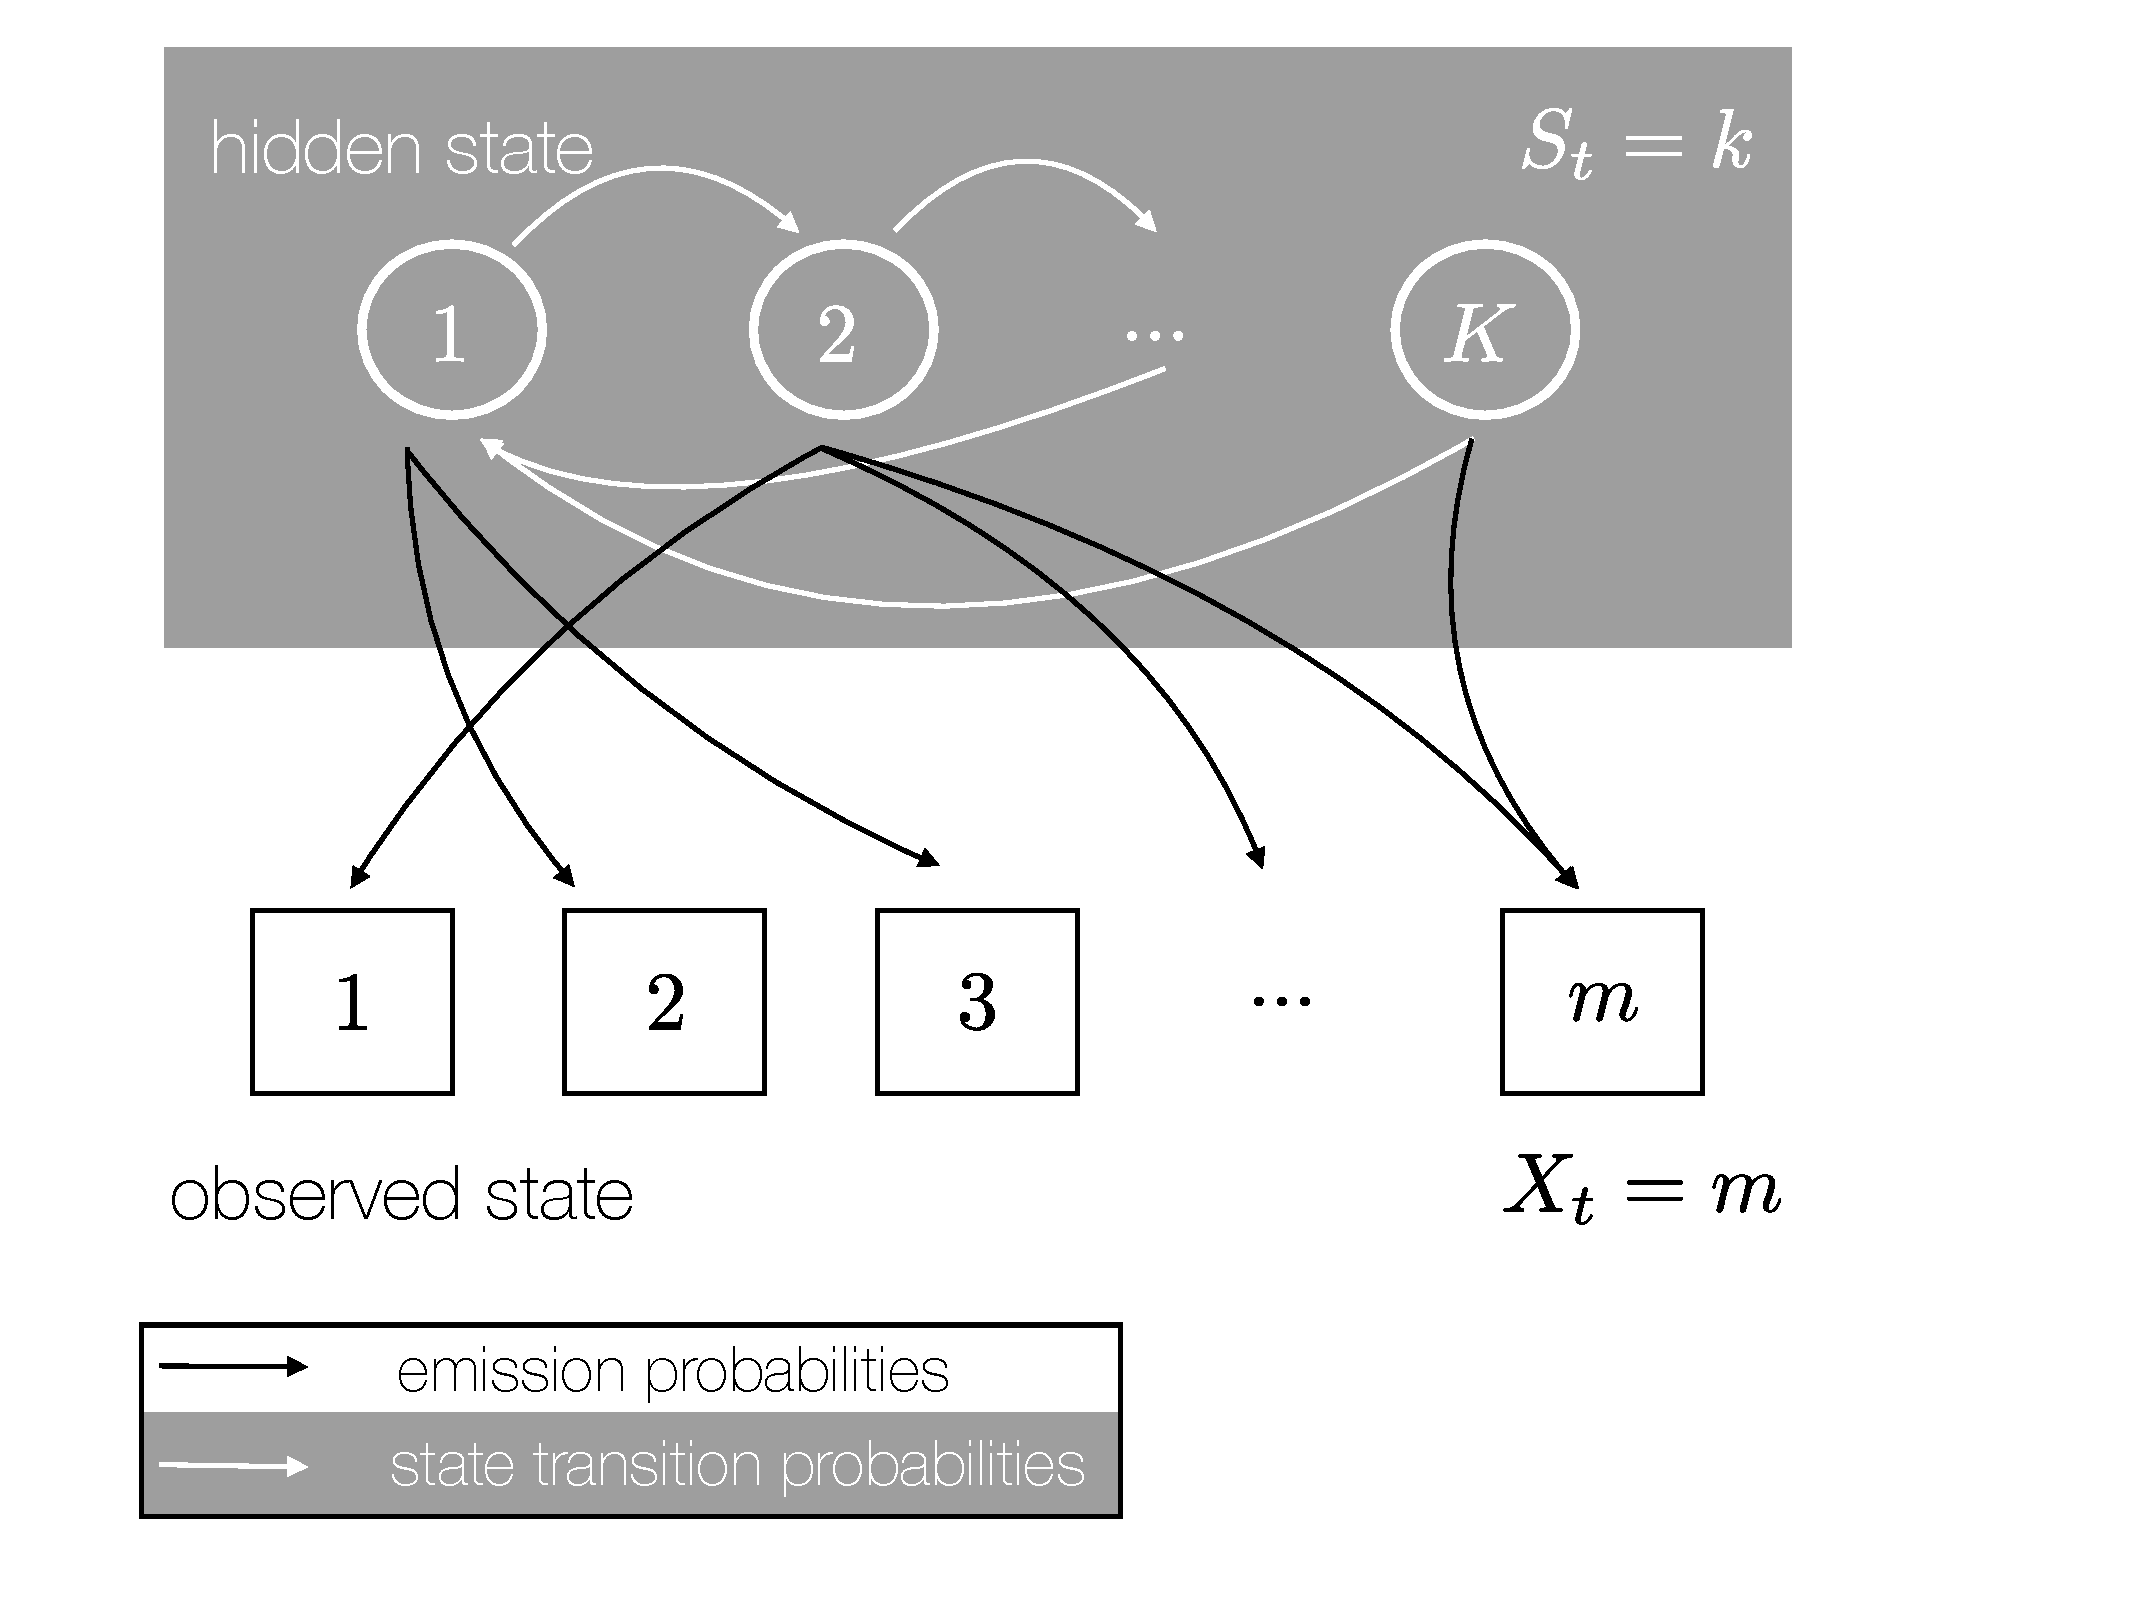
\includegraphics[width=0.8\textwidth]{pics/hmm-schem.pdf}
\caption{Schematic HMM. This diagram shows the general structure of an HMM. The hidden state at time $t$ is $S_t=k$, where $k \in \{1, \ldots, K\}$. The white arrows represent transitions between hidden states. Observed state at time $t$ is characterised by $X_t =m $ for $m \in \{1, \ldots, M\}$. Discrete emissions probabilities from hidden states to observed states are shown as black arrows.}
\label{fig:hmm-schem}
\end{figure}

An extension to Markov chains that has found widespread application in biological systems is the Hidden Markov Model (HMM)  initially developed by \cite{Baum:1966cy}. The big difference to a classical Markov chain is that in an HMM the states of the Markov chain are not directly observed. Instead, observations are made on outputs dependent on the hidden states. The possible observable outputs can be discrete or continuous while the hidden Markov chain has a discrete state space.

More specifically the hidden Markov chain has transition probabilities (as described above) as well as emission probabilities, see Figure \ref{fig:hmm-schem} for a schematic of an HMM. We can write the hidden state process at time $t$ as $S_t$ in discrete time and with a discrete state space i.e. $S_t \in \lbrace 1, \ldots, K \rbrace$ with transition probabilities $p_{i,j} = Pr(S_{t+1} =j | S_t =i)$ and initial probability distribution $p_1 = Pr(S_1 = k)$. Now we write the observation from this hidden Markov chain at time $t$ as $X_t$; here we have to distinguish between two types of outputs that can either be discrete or continuous. If the observation is discrete i.e. $X_t \in \lbrace 1, \ldots, M \rbrace$ we have emission probabilities  $b_k(m) = Pr(X_t = m | S_t = k)$ with $j = 1, \ldots M$. If the observation is continuous i.e. $X_t \in \mathbb{R}^M$ we have to use a continuous probability density function which is usually a weighted sum of Gaussian distributions $b_j(X_t) = \sum_{m=1}^M c_{jm}\mathcal{N}(\mu_{jm}, \Sigma_{jm})$, where $c_{jm}$ is a weighting coefficient.

More information on HMMs can be found in \cite{MacDonald:1997wm} and in \cite{Zucchini:2009vl} including sample applications.


\subsection{Maximum likelihood}
\label{sec:least-squares}

Once the model to be used to analyse data is established the question of parameter estimation arises. The most widely used method in statistics for such a parameter estimation from data is  to write down and maximise the likelihood function

\begin{equation}
  \mathcal{L}(\theta) = p(X = x| \theta) ,
\end{equation}
where $X$ and $x$ are as defined above and $\theta$ is a set of parameters. This likelihood function $p(X = x|\theta)$, is a joint probability density function over all observations $x$ conditional on the parameters $\theta$.  Often it is more convenient to work with the log-likelihood function with $l(\theta) = \log \mathcal{L}(\theta)$. Since the logarithm is a monotone function the maximum of $l (\theta)$ is the same as the maximum of $\mathcal{L} (\theta)$. The advantage of the log-likelihood is that it can be easier to work with as the $\log$ transformation can simplify the likelihood. In some cases it is possible to obtain the maximum likelihood estimator (MLE) $\hat{\theta}$ that maximises $\mathcal{L}(\theta)$ and $\ell (\theta)$ in closed form. Especially in real world applications, this can be difficult or there might not exist a closed form solution; in such cases we need to use a more numerical approach.

To show one such approach we present a simple application of the principles and choose a common statistical model to illustrate the idea. Say there exists a model which predicts the response variable $y$ from a set of input variables $x_1 \ldots x_p$. The illustrative model we choose as an example system is the simple linear regression:

\begin{equation}
  \label{eq:simple-regression}
  y_i = \beta_0 + \beta_1 \, x_{i,1}  + \ldots +\beta_p \, x_{i,p}+ \epsilon_i,
\end{equation}
where $\epsilon_i \sim \mathcal{N}(0, \sigma_i^2)$ is independent of observations, $\beta_j$ are unknown parameters, $y_i$ is the response variable for the $i^{\text{th}}$ sample and $x_{i,1}, \ldots x_{i,p} $ are the predictor variables for the $i^{\text{th}} $ sample. It is often beneficial to write eqn. (\ref{eq:simple-regression}) in vector form and include a $1$ in the $\mathbf{x_{i}} = [1, x_{i1}, \ldots , x_{ip}]$ vector and the $\beta_0$ in the $\mathbf{\beta}$ vector to write $y_i = \mathbf{x}_i^T \mathbf{\beta}$. The maximum likelihood solution can be found by minimising the following equation, which is equivalent to the least squares

% The least squares method proposes finding estimates of parameters by determining the parameter set that minimises
% \begin{equation}
%   \label{eq:rss-ls}
%   RSS(\beta) = (Y - \mathbf{X}^T \mathbf{\beta})^2,
% \end{equation}
% also known as the residual sum of squares equivalent to maximising likelihood. Of course this can be extended to multiple input and variables by computing the sum over all RSS, written in vector notation it is

\begin{equation}
  \label{eq:rss-ls}
  RSS(\beta) = \lVert \mathbf{y} - {x}\boldsymbol{\beta}\lVert^2_2,
\end{equation}
where $\mathbf{y}$ is now a vector over all responses and has length $n$ and ${x}$ is now a matrix with dimensions $n \times (p + 1)$. It is also known as the residual sum of squares (RSS) and is fact sums RSS values for all input variables. This is a very simple way of finding parameters of a model that best describes observations.

\subsection{Regularisation}
\label{sec:penalisation}

It can be of benefit to penalise complex models that contain too many parameters, this will also prevent over-fitting and can help in interpretation of results. One way of achieving this regularisation is to  minimise the log-likelihood subject to a constraint on model parameters. An analogous but easier to implement solution is to minimise the log-likelihood with an additive penalty term on parameters. Choosing the example mentioned in Section \ref{sec:least-squares} we write

\begin{equation}
  \label{eq:pen-log-lik}
  \hat{\boldsymbol{\beta}} = \underset{\boldsymbol{\beta}}{\operatorname{argmin}}  \left\lbrace \lVert \mathbf{y} - x\boldsymbol{\beta}\lVert^2_2 + \lambda\, g(\boldsymbol{\beta}) \right\rbrace,
\end{equation}
where $\lVert  \cdot \rVert_2$ denotes the $\ell_2$ norm, $g(\boldsymbol{\beta})$ is the penalty function on $\boldsymbol{\beta}$ parameters and is chosen depending on application and $\lambda$ is a parameter controlling the strength of the penalty; a larger value corresponds to a stronger penalty. The strength parameter $\lambda$ is generally set by cross-validation, or any other model selection criteria (see below for a discussion of model selection). The penalty term itself can take several forms each favourable in different applications, with the same primary aim of reducing model complexity but with different properties. Here we present two possibilities, ridge regression and Lasso.

In ridge regression the added penalty term takes the form of a $\ell_2$ norm over the parameters $g(\boldsymbol{\beta}) = \lVert \boldsymbol{\beta} \rVert_2^2$. It penalises the magnitude of parameters and also shrinks them towards zero but they are never exactly zero. Another method is least absolute shrinkage and selection operator (Lasso), which has been used before but was reintroduced to the statistics community by \cite{Tibshirani:1996wba}. It uses a $\ell_1$ penalty i.e. $g(\boldsymbol{\beta}) = \lVert \boldsymbol{\beta} \rVert_1$. Just like ridge regression Lasso penalises the magnitude of model parameters and therefore the magnitude of larger positive or negative numbers are shrunk down. The advantage of Lasso over ridge regression is that in addition to penalising higher values of parameters increasing the strength of the penalty forces more and more parameters to be exactly zero reducing model complexity, see \cite{hastie2001elements} for more details.

\subsection{Identifiability}
\label{sec:identifiability-back}

For models where parameters are of physical importance, identifiability plays a crucial role. It is important to remember that the concept of identifiability is a theoretical concept. It does not relate to application of the model to real data but rather refers to the model itself and an application to idealised potentially infinite amount of data which is also noise free. Stating the definition formally, let $M(\theta)$ be a model with a set of parameters $\theta$ from the parameter space $\Theta$. Then we say a model $M(\theta)$ is identifiable when $M(\theta_1) = M(\theta_2)$ holds if and only if $\theta_1 = \theta_2$ for all possible $\theta_1, \theta_2 \in \Theta$. In other words if the model returns the same output for two different parameters it is not identifiable.

More information on identifiability and some applications can be found in \cite{Saccomani:2003kx},  \cite{Saccomani:2010by} and \cite{Jacquez:1985fz}. It is a widely studied subject especially in the context of linear models, but results for nonlinear models are more difficult to obtain.

\subsection{Model selection}
\label{sec:model-selection-1}

The aim of a model is to enable description of a complex (sometimes not even fully understood) phenomenon in a way that they are tractable by mathematics. Statistical or even mechanistic models include in their core assumptions and simplifications of the real world problem they are attempting to describe. In some cases, this can be the only way to describe properties of the system. Often experiments are sufficient to distinguish between models and identify the one closest to the real world problem. There are also cases where due to insufficient data or the type of data available two distinct models appear feasible. This problem is encountered especially when employing statistical models and comparing observed data with predictions from such models. The universal problem then becomes the comparison of model predictions to a set of noisy data. Even in cases where the model itself is identifiable (see discussion above), the existence of noise in observations poses a real difficulty. In such cases the question that one is really trying to answer is one of prediction. Model fit to data is not a sufficient measure. After all, the error between model prediction and a specific data set will not carry over to a different data set; but it is still an important indicator and cannot be discarded.  One wishes to avoid over-fitting as this ensures that prediction not only works for the fitted data but also can be applied more generally.

\subsubsection{Cross-validation}
\label{sec:cross-validation}

One method that uses this idea in a data driven fashion is cross-validation. The basic principle is quite simple, data  is split into two independent subsets (the training set and the validation set) and model parameters are estimated on the training set. Then, predictions using these parameters are compared with the validation set resulting in a performance score. A practical approach is called $k$-fold cross-validation. Here the data set is split into $k$ randomly chosen equally sized subsets, one subset is retained as the validation set and the remaining $k-1$ subsets are used as training data. This step is repeated for each of the $k$ subsets and the performance score is combined giving one score for each model. In some applications such as the ones discussed in later chapters of this work, due to limitations in data it is only feasible to leave out one data point at a time, also called leave-one-out cross-validation. This procedure is then repeated for every model that is considered and the optimal model is chosen based on the best score. It is clear that such an approach has drawbacks; when dealing with large data sets computation times can quickly become infeasible since estimation is repeated for $k$ subsets, for all data and for all possible models. An additional problem can be that due to the random splits in data the choice of the split influences results significantly. Therefore, it is often advisable to try multiple splits and compare results.

\subsubsection{AIC and BIC}
\label{sec:aic}

To avoid lengthy computation time there are many methods to approximate model selection results based on information obtained when estimating parameters, reducing the number of computations to one per model and data. This is an obvious advantage but it is a further approximation hence one has to be careful interpreting results and the choice of approximation used. In all such approaches the goodness of fit is juxtaposed to model complexity i.e. since more complicated models will perform better during estimation for a given data set we want to penalise models dependent on the complexity of the model. Such methods due to historical naming convention are referred to as information criteria. Here we will briefly introduce two such models. One of the most widespread is the Akaike information criterion (AIC) formulated by \cite{Akaike:1974ih} and the other is the Bayesian information criterion (BIC) presented by \cite{Schwarz:1978uv}. AIC is computed using the log-likelihood $l(\theta)$ for model parameters $\theta$ and the degrees of freedom $d$:

\begin{equation}
  \label{eq:aic-def}
  AIC = -2 \;l(\theta) + 2 d.
\end{equation}
It is derived using ideas in information theory namely the Kullback-Leibler divergence between the true model for a data set and the used model. When dealing with small sample sizes this measure is not satisfactory and is replaced by the corrected version the AICc. It adds an additional term dependent on sample size $n$
\begin{equation}
 AICc = -2 \; l(\theta) +2d + (2 * d (d + 1)) / (n - d - 1).
\end{equation}


The other information criterion, the BIC is derived using a Bayesian approach. It is also applied for a log-likelihood approach just like AIC. The derivation of BIC starts with the assumption that there exists a posterior distribution for models $M_i$ given some data $\mathbf{y}$ written $P(M_i| \mathbf{y})$. Here we introduce a subscript for models to easily label different models as the difference will not only be the parameters. Using Bayes' theorem we can write the odds of two models as:

\begin{equation}
  \label{eq:bic-odds}
  \frac{P(M_i|\mathbf{y})}{P(M_j|\mathbf{y})} = \frac{P(M_i)}{P(M_j)} \cdot \frac{P(\mathbf{y}|M_i)}{P(\mathbf{y} |M_j)}.
\end{equation}
The final term in eqn. (\ref{eq:bic-odds}), the ratio of marginal likelihoods, is also known as the Bayes factor. The prior over models is typically assumed to be flat, then $P(M_i) = P(M_j)$ for all $i$, $j$ the right-hand side of eqn. (\ref{eq:bic-odds}) just reduces to the Bayes factor. To approximate the marginal likelihood $P(\mathbf{y} | M)$ we use the Laplace approximation which is a method to approximate integrals. It yields the BIC score for a given model with parameters $\theta$:

\begin{equation}
  \label{eq:bic-def}
  BIC = -2 \; l(\theta) + \log(n) \,d.
\end{equation}
The penalty for complex models in BIC is larger than in AIC hence it will select for simpler models. Additionally as sample size $n\rightarrow \infty$ and the model space includes the true model BIC will select the correct model, i.e. it is asymptotically consistent unlike AIC. However, AIC will sometimes perform better for smaller sample sizes \citep{hastie2001elements}. Hence the decision of information criterion will be application dependent.

\subsection{Monte Carlo integration}
\label{sec:monte-carlo-integr}

In many applications of mathematical models to real world problems one encounters integrals without closed form solutions. For such cases numerical methods, which have become particularly wide spread since advancements in computational power, allow for large-scale computations in relatively short time. Monte Carlo integration is one such example. Generally, Monte Carlo techniques are ubiquitous for classes of problems which include random numbers.

If we have a function $f(X)$ of a random variable $X$  which is uniformly distributed between $a$ and $b$, we can write the expectation of $f(X)$ as the integral
\begin{equation}
  \label{eq:mc-integ-def}
  E(f(X)) = \frac{1}{b-a} \int_a^b f(x) dx,
\end{equation}

The law of large numbers states that the sum of $n$ random variables divided by $n$ converges to the expected value of the random variable as $n \rightarrow \infty$. This is a very powerful idea and since we know that the function of a random variable is also a random variable we can extend this to the function of a random variable $f(X)$.  As the number of samples $n$ taken from random variable $X$ approaches infinity

\begin{equation}
  \label{eq:mc-larg-num}
  \frac{1}{n} \sum_{i=1}^n f(X_i) \rightarrow \frac{1}{b - a}\int_a^b f(x) dx \hspace{1cm}   \text{as } \: n \rightarrow \infty.
\end{equation}
The left hand side of eqn. (\ref{eq:mc-larg-num}) is therefore an asymptotically consistent estimator of the expectation of $f(X)$ i.e. it converges to the right hand side as $n \rightarrow \infty$. Eqn. (\ref{eq:mc-larg-num}) is the Monte Carlo estimate of an integral and an important issue to always bear in mind for this method is convergence, as without the result having converged sufficiently, they are meaningless. Therefore, in applications the shape of the probability distribution of $X$ plays a central role in determining how well the Monte Carlo integral will converge. This means if function $f(X)$ has a large weight for a value of $X$ which is unlikely to be sampled then for finite $n$ the estimate will be bad. In general for finite $n$ the solution will only be approximate as proper convergence is not possible for finite $n$. More information on Monte Carlo integration can be found in the review article by \cite{James:mc}  and in \citet[Chapter~5]{norris1998markov}.

%%% Local Variables:
%%% TeX-master: "warwickthesis"
%%% End:
